\section{Pengujian dan Pembahasan}
\label{sec:pengujian}

Proyek \textit{capstone} sistem deteksi manusia memerlukan beberapa pengujian untuk mengetahui kualitas sistem. Pengujian dilakukan pada dasarnya untuk mengetahui keberhasilan proyek mengeksekusi perintah pada setiap tahap. Hal-hal yang perlu diketahui dari sistem antara lain yaitu keberhasilan sistem membaca denah ruangan dengan \lidar, mendeteksi bentuk garis dan lingkaran, dan mendeteksi posisi manusia di ruangan tersebut.

\subsection{Skenario Pengujian Simulasi \lidar\ dan Analisis}
\label{subsec:Skenario51}
Gambar denah ruangan beserta posisi manusia dipersiapkan sebagai nilai masukkan simulasi sensor. Denah ruangan akan diubah menjadi data dua dimensi dengan cara memindai warna tertentu dan mencatat lokasi pixel gambar tersebut. Gambar denah memiliki objek berwarna hitam dan ruang kosong berwarna putih seperti Gambar \ref*{fig:Ch05_denah}.
\begin{figure}[H]
    \centering
    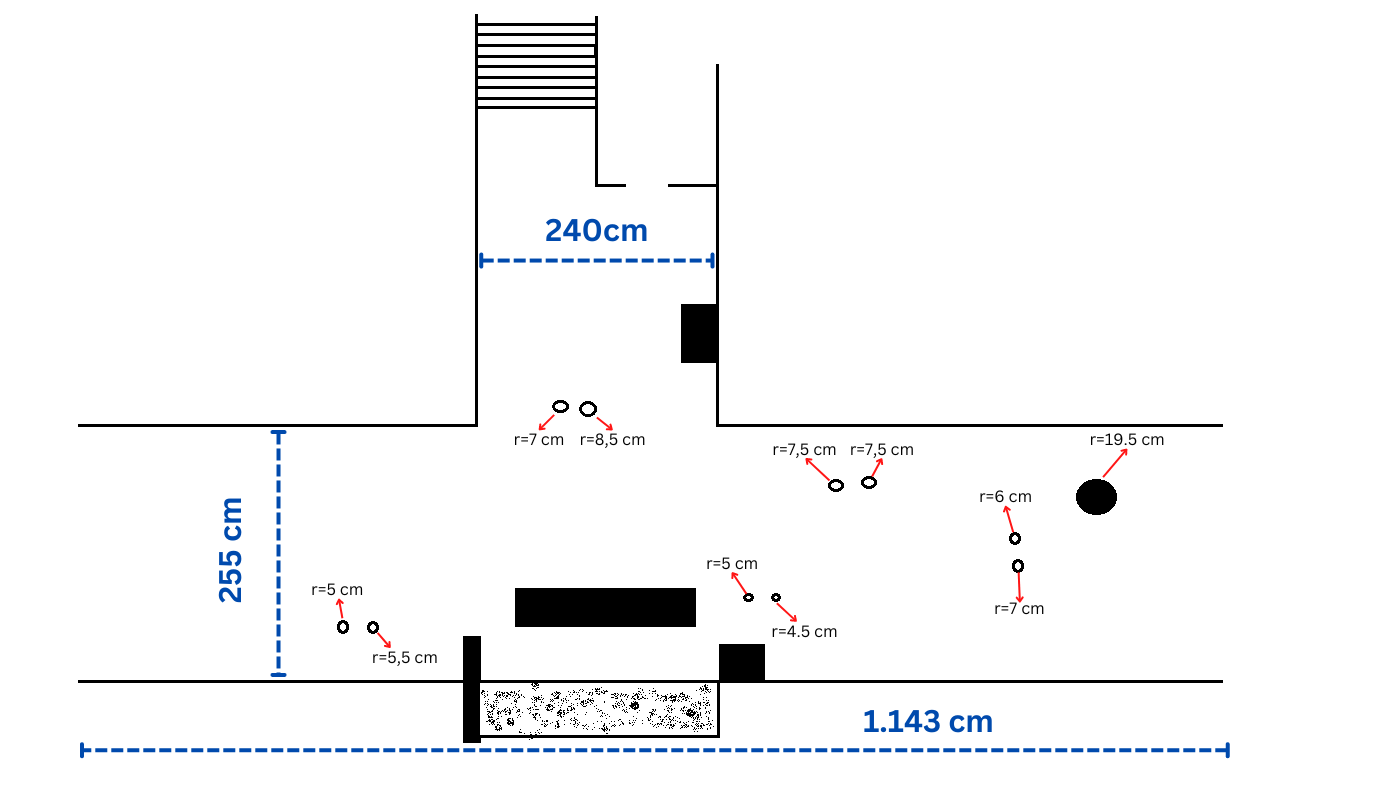
\includegraphics[width=\linewidth]{bab5/map_autotest.png}
    \caption{Gambar Denah Ruangan.}
        \label{fig:Ch05_denah}
\end{figure}

Denah ruangan berisi tembok, benda mati, dan kaki manusia yang berupa dua buah lingkaran kecil berdekatan. Ukuran-ukuran lebar ruangan, kaki manusia dan objek lingkaran lainnya terlihat pada gambar. Terdapat lima pasang kaki manusia dengan diameter kaki berkisar antara 9 cm hingga 17 cm. Data ruangan kemudian dipindai oleh program \lidar\ yang menghasilkan tampilan ruangan seperti pada Gambar \ref*{fig:Ch05_denahbacaan}.
    \begin{figure}[H]
        \centering
        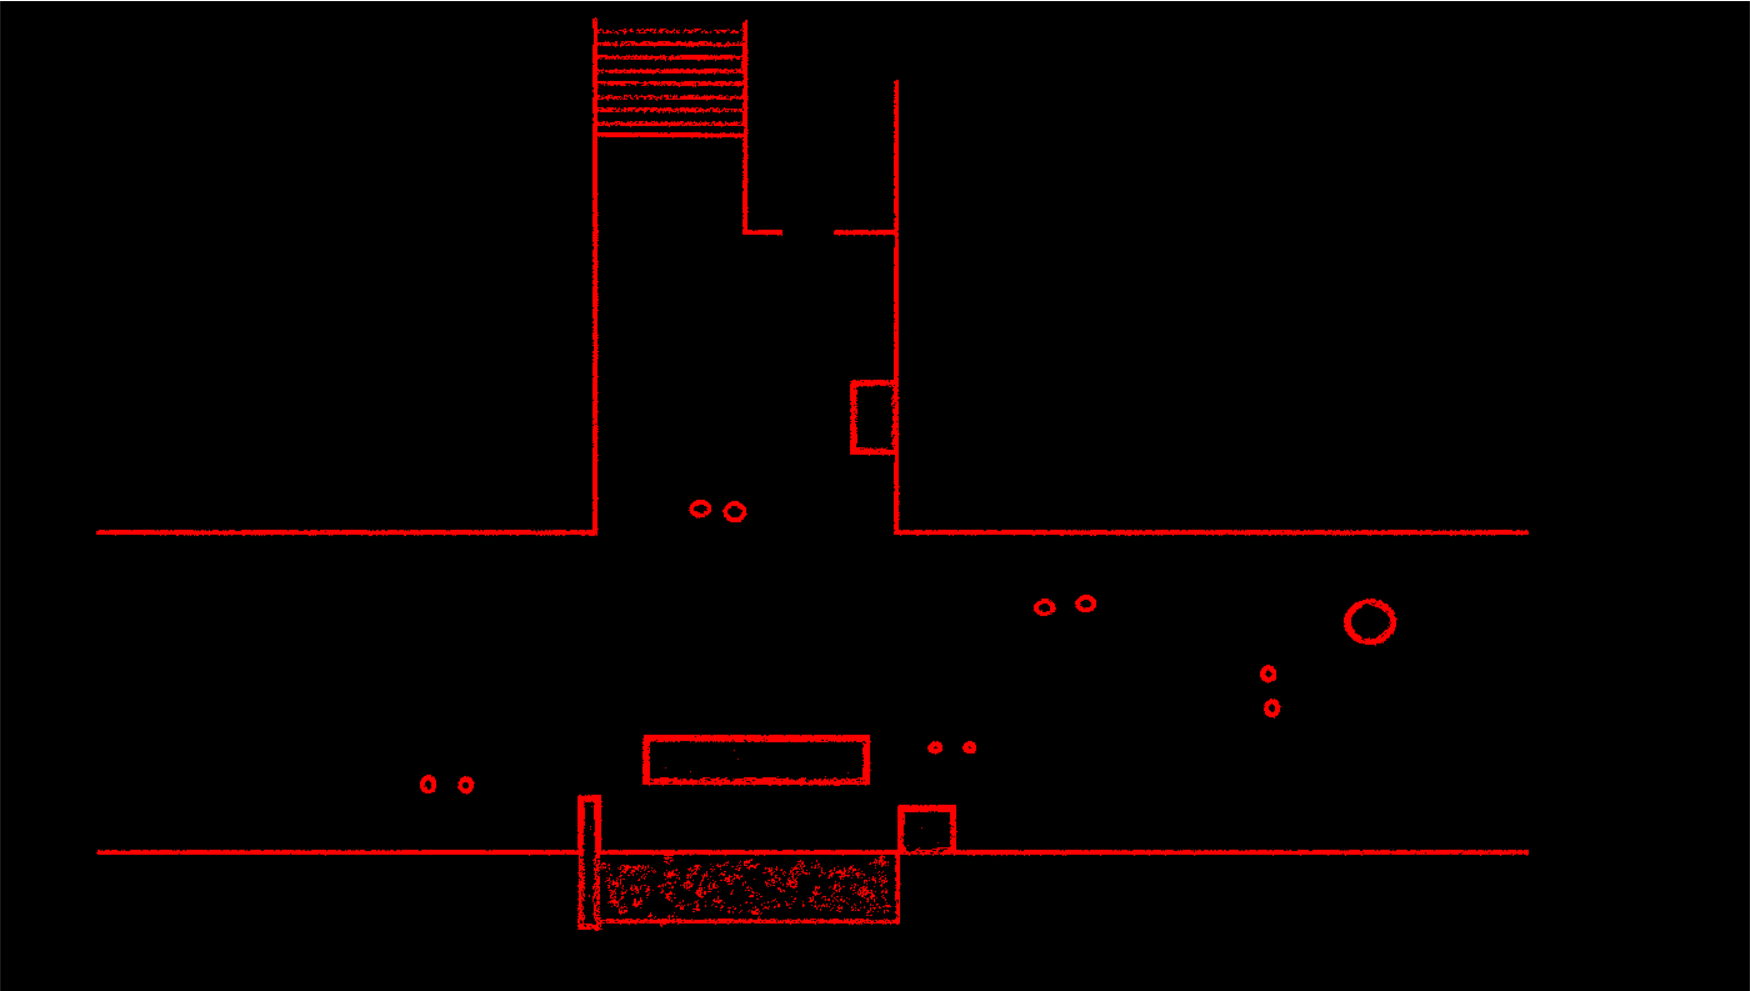
\includegraphics[width=.9\linewidth]{bab5/map_bacaan.png}
        \caption{Gambar Hasil Bacaan Program pada Denah.}
        \label{fig:Ch05_denahbacaan}
    \end{figure}
Data tersebut masih belum memiliki \textit{error}. Simulasi pembacaan sensor \lidar\ juga memerlukan beberapa ketentuan agar mirip dengan pembacaan \lidar\ yang sesungguhnya. 
Spesifikasi \lidar\ yang digunakan program  ditunjukkan pada Tabel \ref*{tab:Ch05_Contoh_Spesifikasi_Luaran}\cite{e1}.
\begin{table}[H]
    \caption{Spesifikasi \lidar\ untuk Simulasi} 
    \label{tab:Ch05_Contoh_Spesifikasi_Luaran} 
    \centering
     \vspace{-0.75em}
   \begin{tabular}{|L{4cm}|L{4cm}|L{4cm}|}
   \hline
   \multicolumn{1}{|c|}{\textbf{Fitur \lidar}} 
   & \multicolumn{1}{|c|}{\textbf{Spesifikasi Asli}} 
   & \multicolumn{1}{|c|}{\textbf{Spesifikasi Simulasi}}
   \\ \hline
    Jarak Deteksi 
      & \multicolumn{1}{|c|}{\makecell{Minimum 15 cm \\Maksimum 8 m}}
      & \multicolumn{1}{|c|}{\makecell{Maksimum 2 m}}
      \\ \hline
    Sudut Deteksi Deteksi 
        & \multicolumn{1}{|c|}{$\ang{0}$ sampai $\ang{360}$}
        & \multicolumn{1}{|c|}{$\ang{0}$ sampai $\ang{360}$}
        \\ \hline
    \textit{Error} Pembacaan Jarak
        & \multicolumn{1}{|c|}{$<1\%$ dari jarak asli \lidar\ ke objek}
        & \multicolumn{1}{|c|}{$1\%$ dalam 1 m}
         \\ \hline
    Jumlah Sampel dalam Satu Putaran
         & \multicolumn{1}{|c|}{400 sampel}
         & \multicolumn{1}{|c|}{400 sampel}
         \\ \hline
   \end{tabular}
   \end{table}
% sensor dibuat dengan masukkan jarak, map, dan uncertainty. uncertainty menambahkan = define uncertainty using covariance and gaussian distribution
% ada uncertainty, gaussian dis, covariance diambil diagonal dari sigma kuadrat. Nanti jarak asli bakal tambah error.
% Data denah ruangan setelah ditambah error bacaan:
Data denah ruangan yang telah diberi error $1\%$ dari jarak aslinya terlihat pada Gambar \ref*{fig:Ch05_denaherror}. Terlihat persebaran titik-titik objek lebih terhambur secara acak dibanding data mentah denah pada Gambar \ref*{fig:Ch05_denahbacaan}.
\begin{figure}[H]
    \centering
    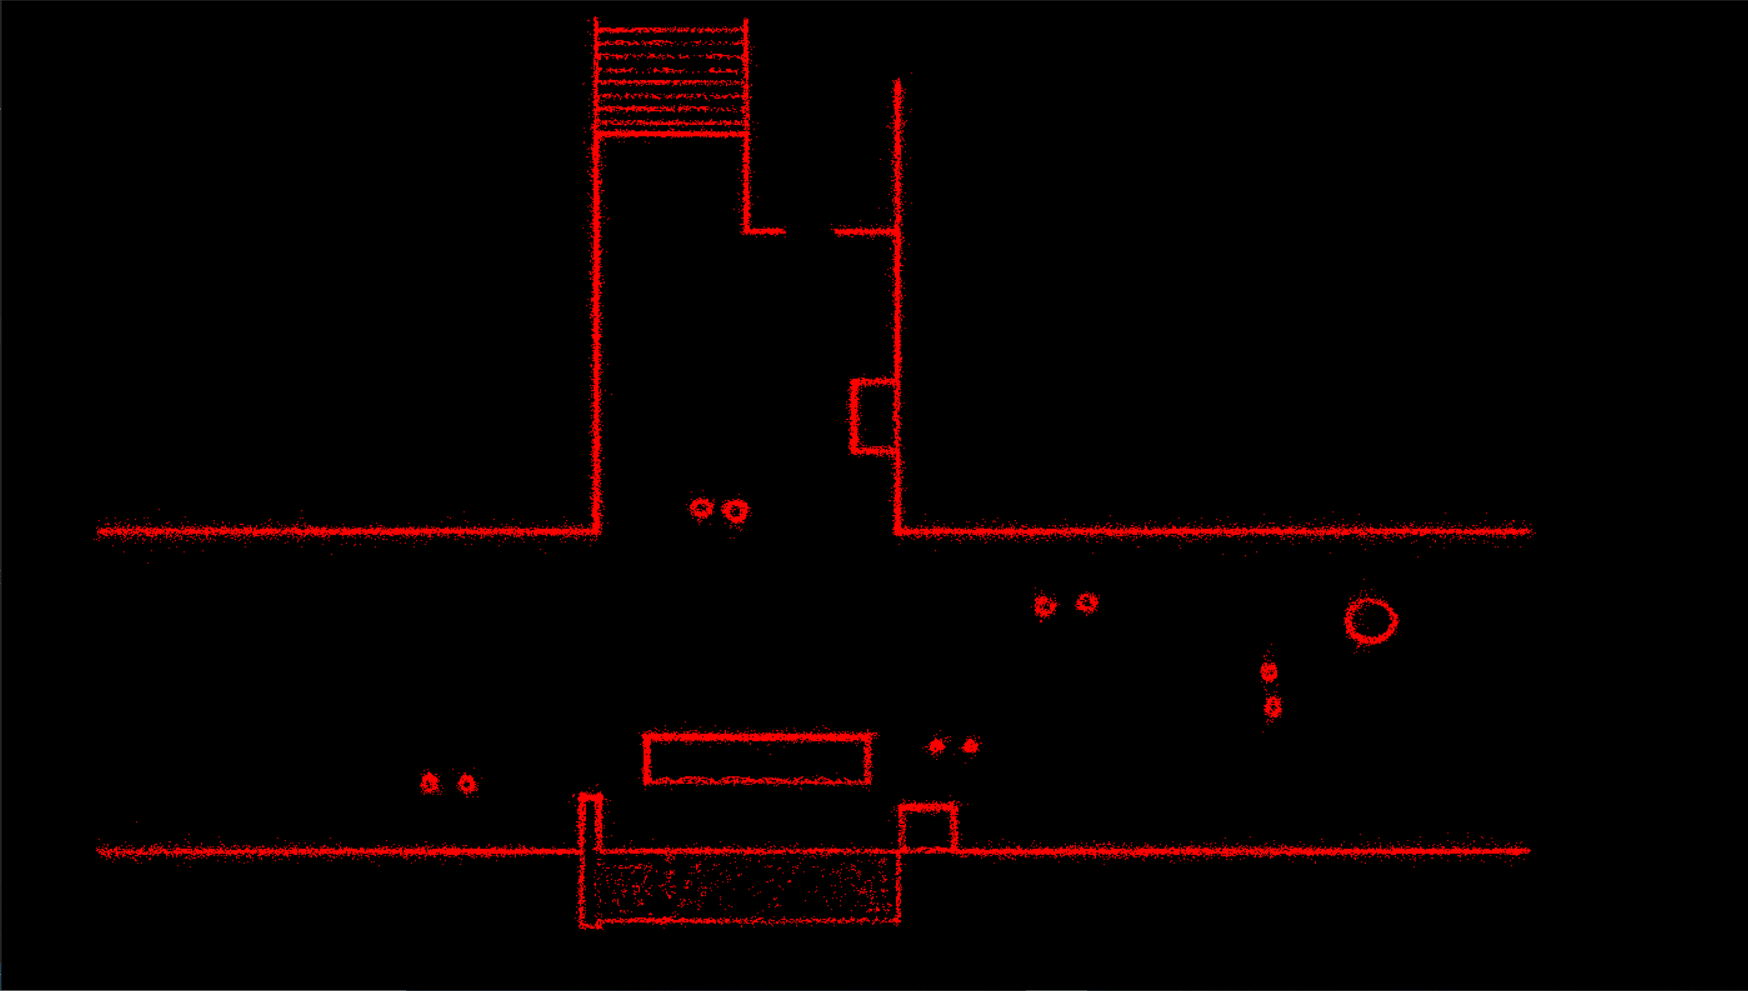
\includegraphics[width=.9\linewidth]{bab5/maperror.png}
    \caption{Gambar Hasil Bacaan dengan \textit{Error}.}
        \label{fig:Ch05_denaherror}
\end{figure}
Hasil pembacaan denah ruangan dengan \lidar\ pada robot bergerak terlihat pada Gambar \ref*{fig:Ch05_bacarobot}. Robot bergerak dari ujung kiri ruangan menuju ujung kanan. Data yang terbaca setiap langkah robot disimpan kemudian ditampilkan. Semakin jauh posisi objek dari \lidar\ maka semakin sedikit tembakkan sinar \lidar\ sehingga data posisi yang diterima juga semakin sedikit. \lidar\ hanya akan memindai permukaan objek yang menghadap \lidar\ sehingga bentuk objek tidak sepenuhnya diketahui oleh robot.
\begin{figure}[H]
    \centering
    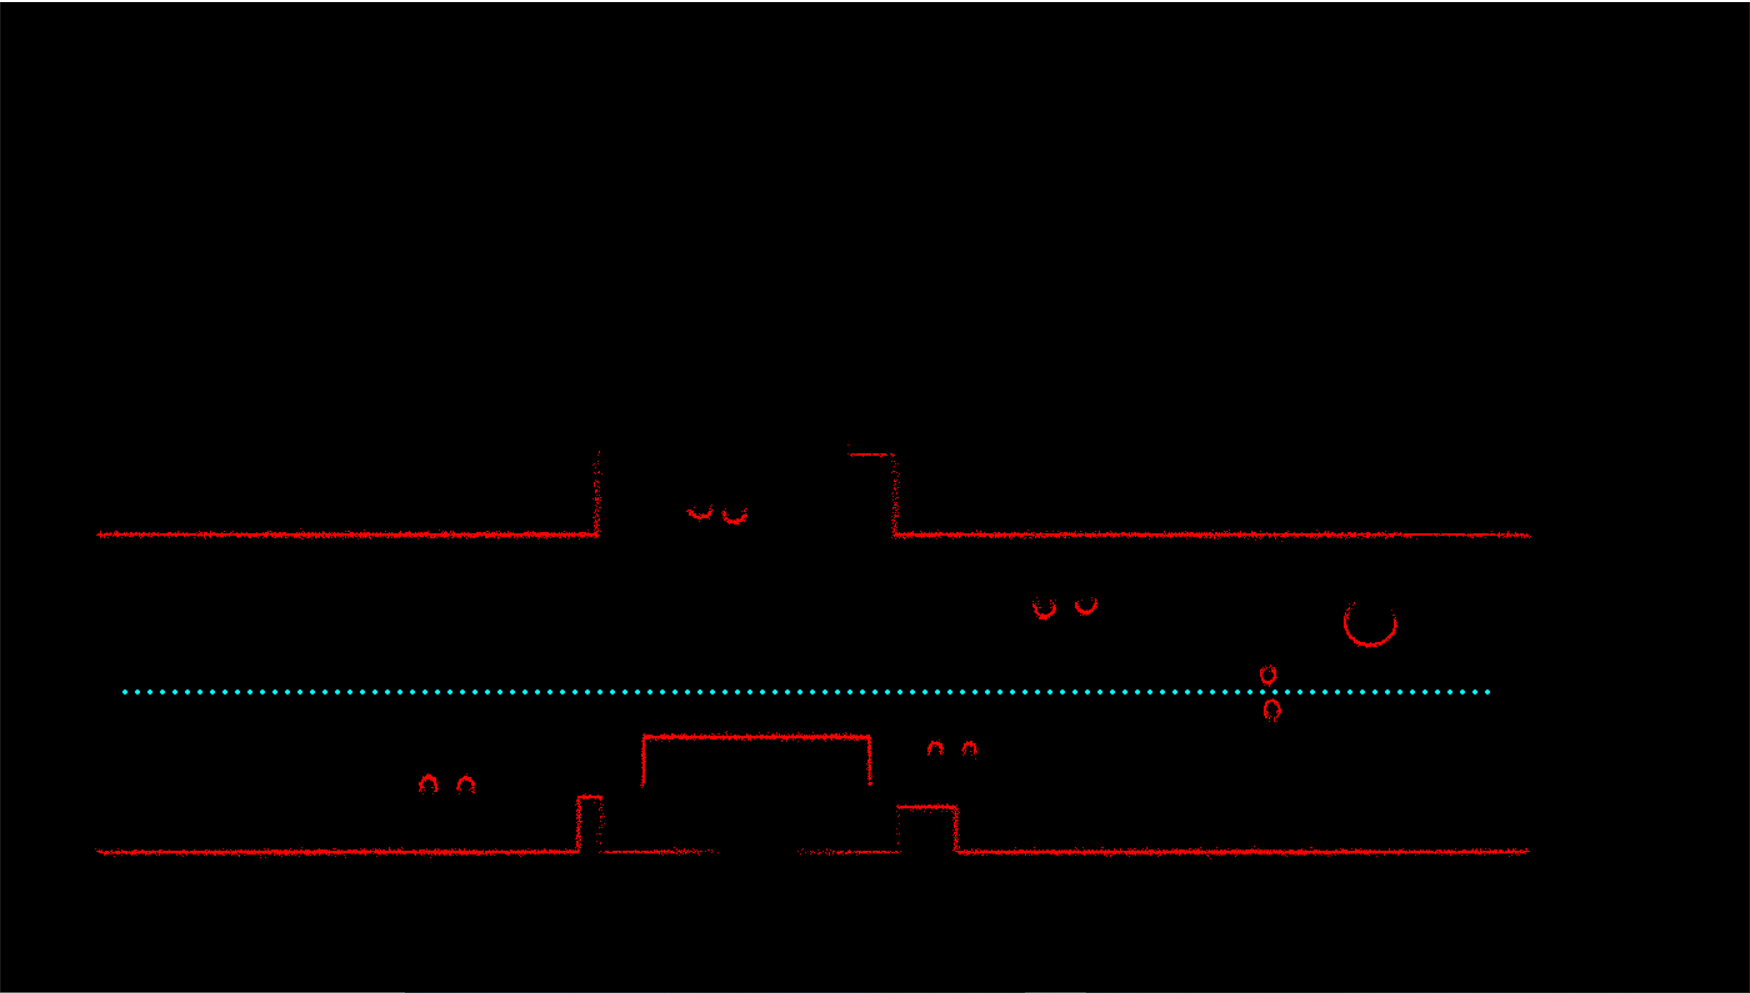
\includegraphics[width=.9\linewidth]{bab5/bacarobot.png}
    \caption{Gambar Bacaan \lidar\ pada Robot Berjalan.}
        \label{fig:Ch05_bacarobot}
\end{figure}
% Model : YDLIDAR X4
% Distance Range:
% minimum: 12 cm 
% maximum: 10 meter 
% Angular Range: 0 - 360º
% Distance Resolution:
% Typical: 2 cm range <= 1 m, 3.5 \% 1m<range<=6 m
% Angular Resolution: (6,7,12 Scan Rate)
% Minimum: 0.43º
% Typical: 0.5º
% Maximum: 0.86º
% Ranging 5000 times per 
% second, motor freq (6-12)
% RPLIdar A2 400 scan:

% Model: RPLDIAR-A2M8
% Distance Range:
% minimum: 15 cm (based on white object with 70% reflectivity)
% maximum: 8 meter (based on white object with 70% reflectivity)
% Angular Range: 0 - 360º
% Distance Resolution:
% Typical: < 0.5 mm, within 1.5 meters of scanning range
% < 1% of the distance for all range
% Angular Resolution: (10Hz Scan Rate)
% Minimum: 0.45º
% Typical: 0.9º
% Maximum: 1.35º
% Sample Duration:
% Typical: 0.25 milisecond (ms)
% Sample Frequency:
% Minimum: 2000 Hz
% Typical: 4000 Hz
% Maximum: 4200 Hz
% Scan Rate: (The rate is for a round of scan. The typical value is measured when RPLIDAR takes 400 samples per scan)
% Minimum: 5Hz
% Typical: 10Hz
% Maximum: 15Hz

% simulasi dilakukan dengan spesifikasi blabla menghasilkan 
% Terlihat dari gampar denah asli di gambar xx, hasil output bacaan lidar menunjukkan titik2 terbaca disekitar obstacles. titik yang terlihat sesuai kondis denah nput dan spesifikasi \lidar.

\subsection{Skenario Pengujian \textit{Fitting Algorithm} dan Analisis}
\label{subsec:Skenario52}

Tahap penting dari sistem deteksi ini adalah menemukan segmen-segmen garis dan lingkaran dari data yang telah dibaca. Perlu diketahui kemampuan pendeteksi bentuk yang telah dibuat. Pengujian ini dilakukan dengan memberi sejumlah titik-titik acak dengan jumlah yang sedikit hingga banyak kemudian dimasukkan ke dalam algoritma \textit{fitting}. Terlihat pada Gambar \ref*{fig:Ch05_P_circfit} dan \ref*{fig:Ch05_P_linefit} bahwa program berhasil mencari bentuk garis yang sesuai dengan data yang diberi. Program menggunakan seluruh titik yang diberi untuk menentukan luaran bentuk garis dan lingkaran. Pada gambar-gambar tersebut juga terdapat dua nilai residu yaitu residu persamaan garis asal dengan residu persamaan garis baru. Residu dicari dengan menjumlahkan jarak terdekat titik dengan garis.
\begin{figure}[H]
    \centering
    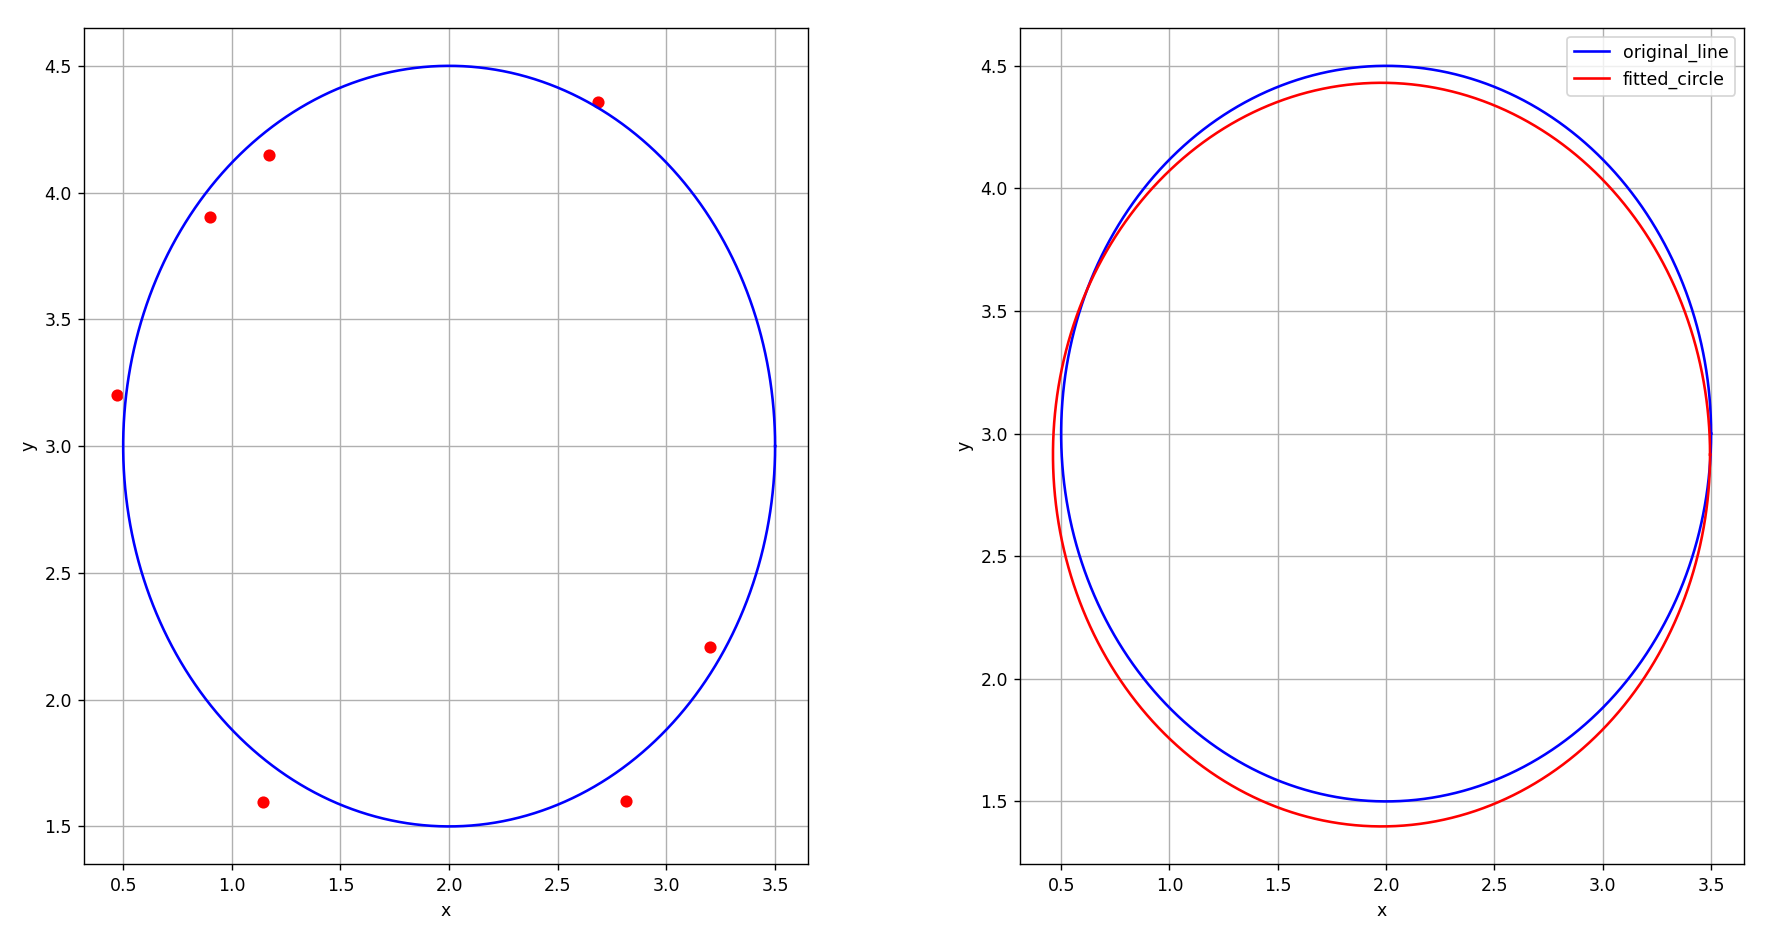
\includegraphics[width=.8\linewidth]{bab5/contoh_Circlefit.png}
    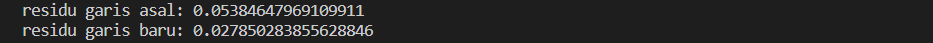
\includegraphics[width=\linewidth]{bab5/residu_Circlefit.png}
    \caption{Pengujian \textit{Circle Fitting}.}
        \label{fig:Ch05_P_circfit}
\end{figure}

\begin{figure}[H]
    \centering
    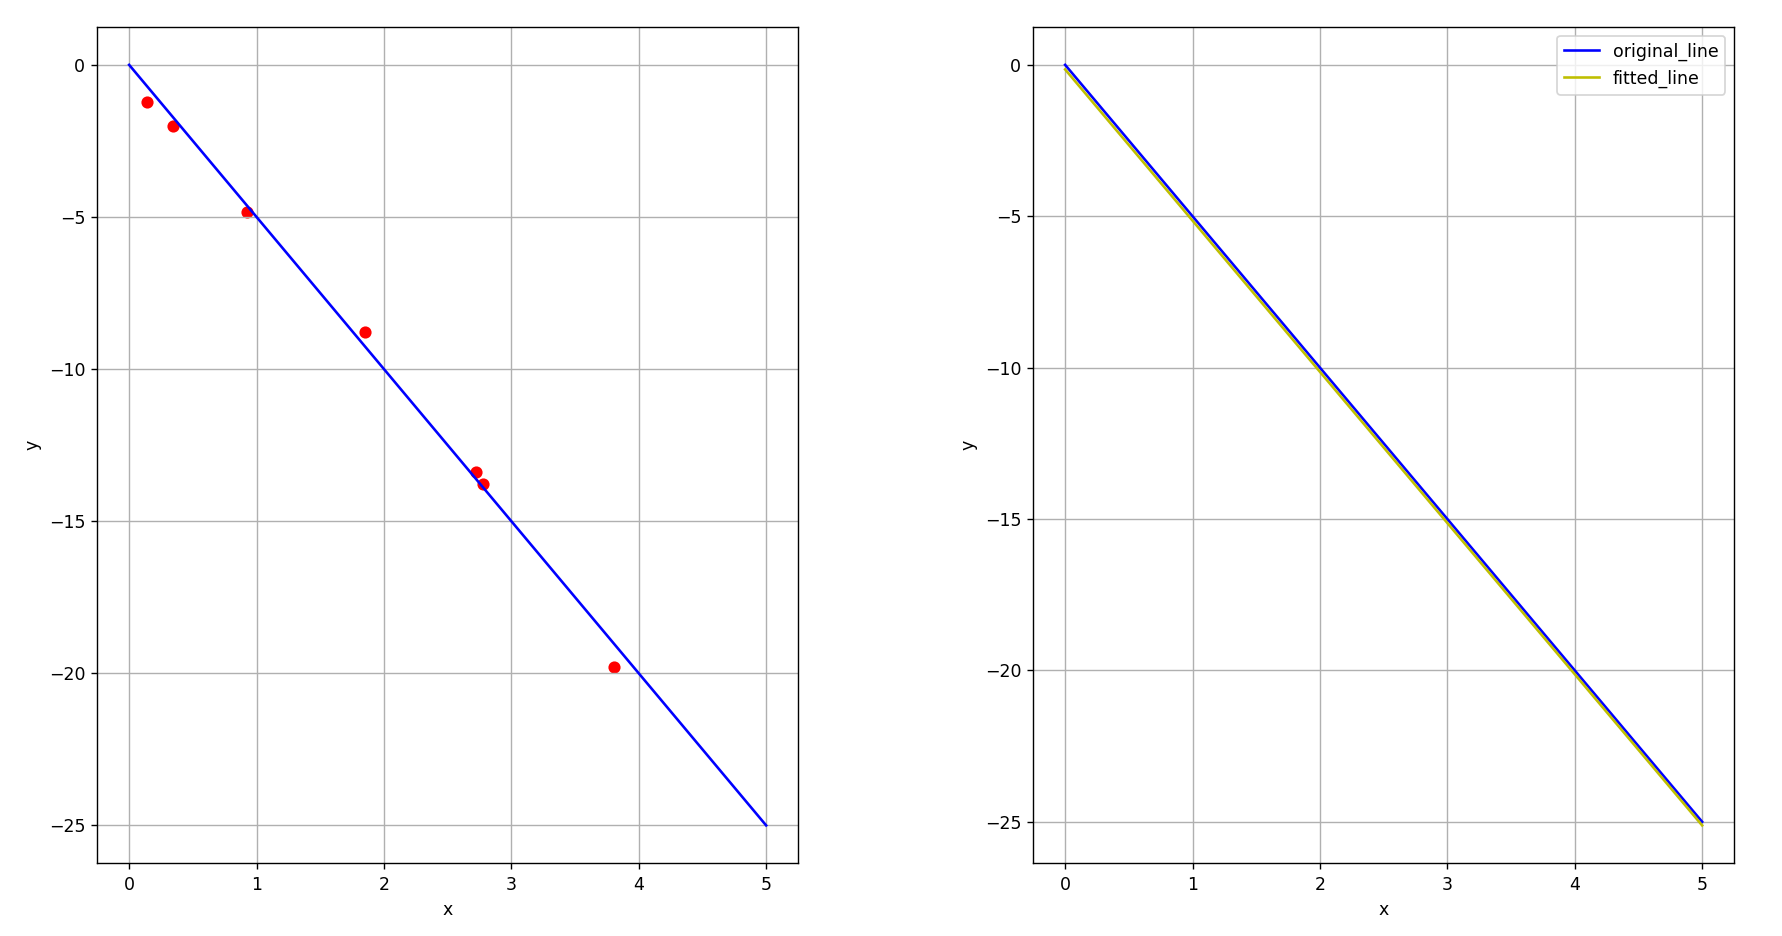
\includegraphics[width=.8\linewidth]{bab5/Contoh_linefit.png}
    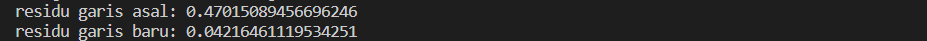
\includegraphics[width=\linewidth]{bab5/residu_linefit.png}
    \caption{Pengujian \textit{Line Fitting}.}
        \label{fig:Ch05_P_linefit}
\end{figure}
Pada kedua gambar terlihat bahwa program berhasil mencari garis baru yang sama bentuknya dengan garis asal berwarna biru.
Perbedaan posisi garis asal dengan garis hasil deteksi disebabkan karena persebaran data yang acak. Kedua algoritma menghasilkan persamaan garis baru yang memiliki residu lebih rendah daripada persamaan garis asal. Hal ini berarti bahwa program berhasil mencari persamaan garis yang paling sesuai dari data yang ada. 

Pengujian dilanjutkan dengan melakukan \textit{circle fitting} dan \textit{line fitting} untuk berbagai jumlah data dari 5 titik hingga 400 titik masukkan. Setiap jumlah titik dilakukan pengujian sebanyak 10 kali kemudian dihitung rata-rata waktu yang diperlukan. Grafik waktu yang dibutuhkan untuk setiap pemrosesan data dapat dilihat pada Gambar \ref*{fig:Ch05_time_consump}.
\begin{figure}[H]
    \centering
    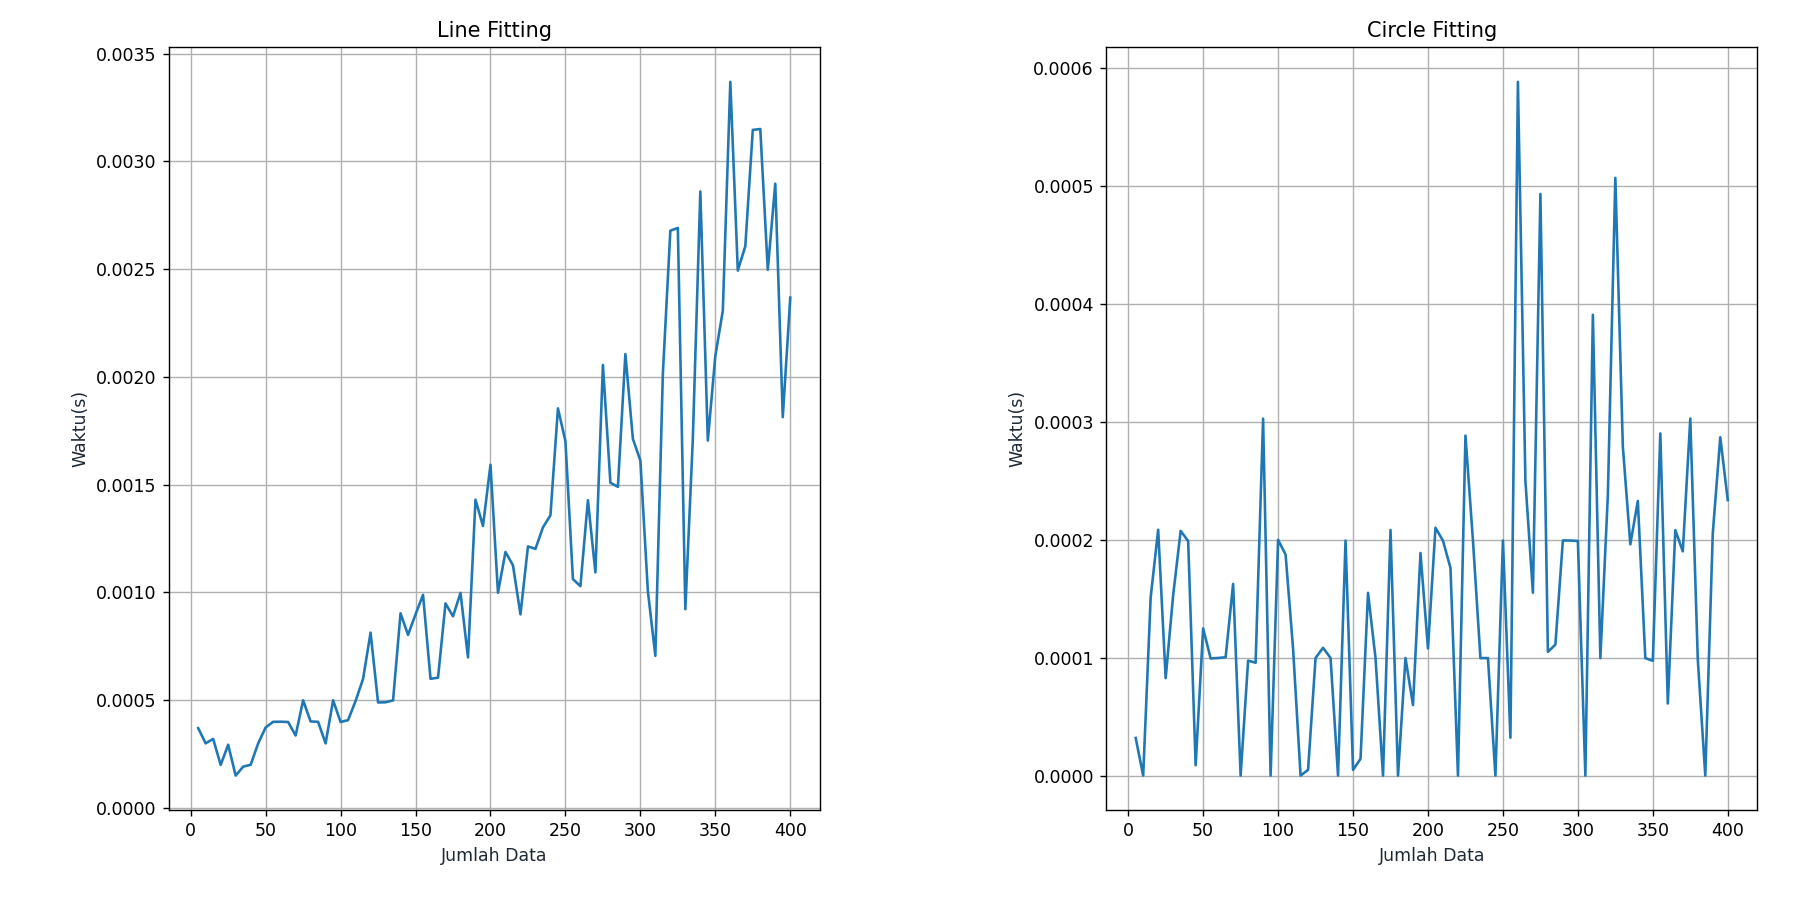
\includegraphics[scale=0.4]{bab5/time_consump.png}
    \caption{Grafik Waktu Pemrosesan}
        \label{fig:Ch05_time_consump}
\end{figure}
Data waktu pemrosesan kemudian dianalisis untuk masing-masing jenis algoritma \textit{fitting}. Hasil analisis diperlihatkan pada Gambar \ref*{fig:Ch05_hasil_time_consump} yang menunjukkan luaran analisis data yang diperoleh. 
\begin{figure}[H]
    \centering
    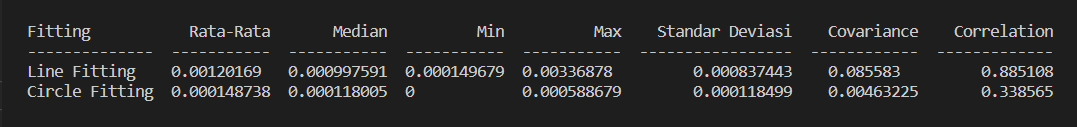
\includegraphics[width=\linewidth]{bab5/hasil_time_consump.png}
    \caption{Data Hasil Analisis Waktu Pemrosesan}
        \label{fig:Ch05_hasil_time_consump}
\end{figure}
\noindent Pada gambar tersebut terlihat berbagai nilai analisis waktu yang diperlukan masing-masing algoritma seperti rata-rata waktu, median, waktu diperlukan paling sedikit, waktu diperlukan paling banyak, nilai deviasi standar, \textit{covariance} waktu dengan data, dan \textit{correlation} waktu dengan data. \textit{Correlation} menunjukkan hubungan antara waktu diperlukan dengan banyak data yaitu semakin mendekati angka 1 maka kedua berarti perubahan banyak data mempengaruhi perubahan waktu yang diperlukan dan semakin mendekati 0 maka berarti variabel waktu dengan jumlah data saling independen.

\subsection{Skenario Pengujian \textit{Seed Detection} dan Analisis}
\label{subsec:Skenario53}

Pengujian tahap ini bertujuan mengetahui keberhasilan proses pencarian segmen awal menggunakan data yang diterima. Pengujian dilakukan dengan menjalankan \lidar\ menuju sebuah objek lingkaran dan objek garis kemudian menyimpan data yang diterima. Lingkaran yang digunakan untuk pengujian memiliki radius bernilai 5 cm. Data tersebut diproses menggunakan algoritma \textit{fitting} untuk mengetahui nilai $\delta$ dan $\epsilon$ minimal yang dimiliki objek. Proses pendeteksian dengan \lidar\ dan objek terlihat pada Gambar \ref*{fig:Ch05_proses_seed}. Robot berjalan dari jarak sekitar 1 m menuju objek dengan perpindahan sebesar 5 cm kemudian data yang diterima setiap perpindahan akan disimpan dengan format yang ditampilkan Gambar \ref*{fig:Ch05_csv_seed}.
\begin{figure}[H]
    \centering
    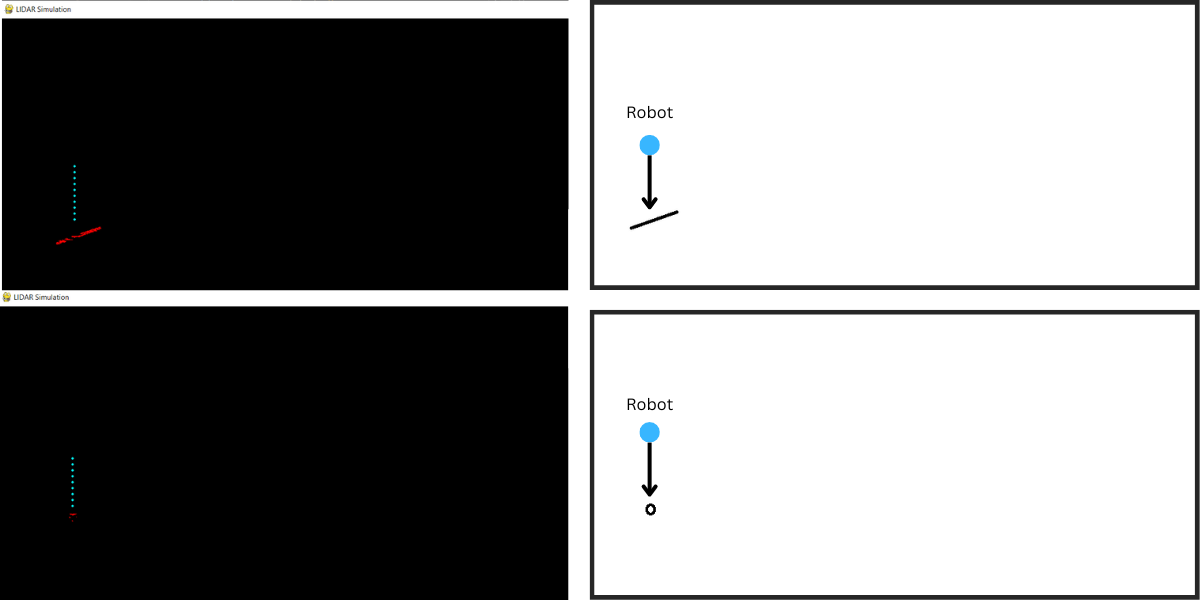
\includegraphics[width=\linewidth]{bab5/proses_seed.png}
    \caption{Proses Pengujian Seed Detection}
        \label{fig:Ch05_proses_seed}
\end{figure}
Perhitungan nilai $\delta$ dan $\epsilon$ dilakukan dari titik pertama hingga titik terakhir dari semua data yang diterima setiap jarak robot dengan objek. Variabel-variabel yang dicari dalam pengujian ini yaitu jumlah titik, $\delta$ tertinggi, $\epsilon$ tertinggi, dan rata-rata radius lingkaran yang terbaca.
\begin{figure}[H]
    \centering
    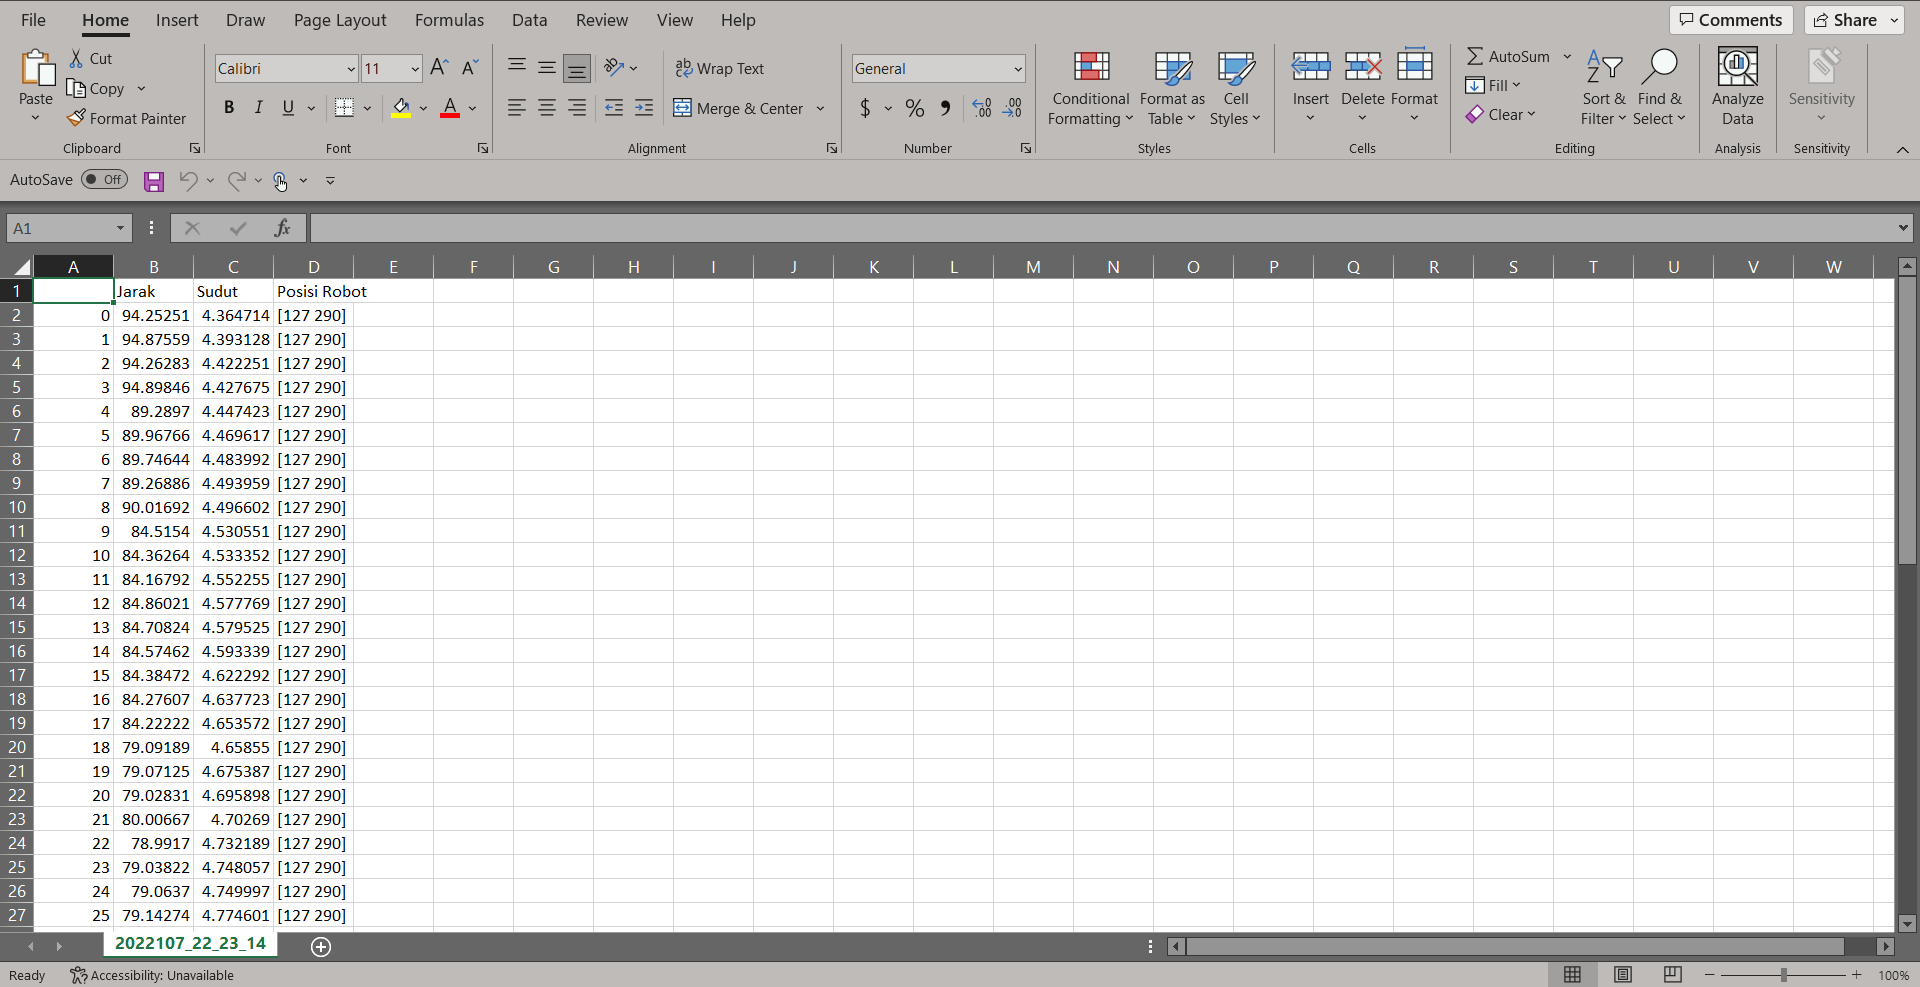
\includegraphics[scale=0.37]{bab5/csv_file.png}
    \caption{Data Luaran Pengujian \textit{Seed Detection}}
        \label{fig:Ch05_csv_seed}
\end{figure}
\begin{figure}[H]
    \centering
    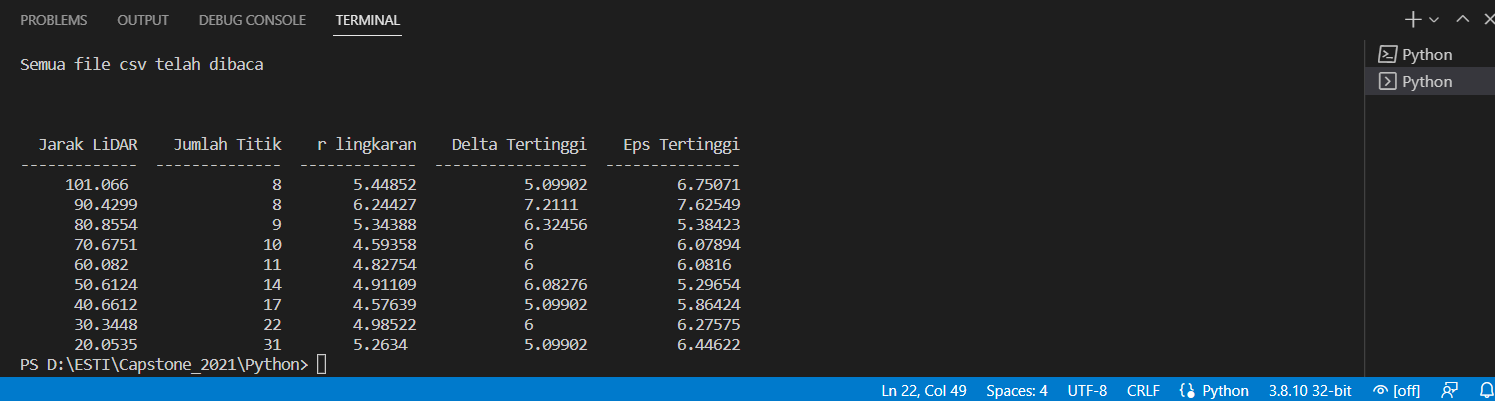
\includegraphics[scale=0.4]{bab5/seed_circle_vars.png}
    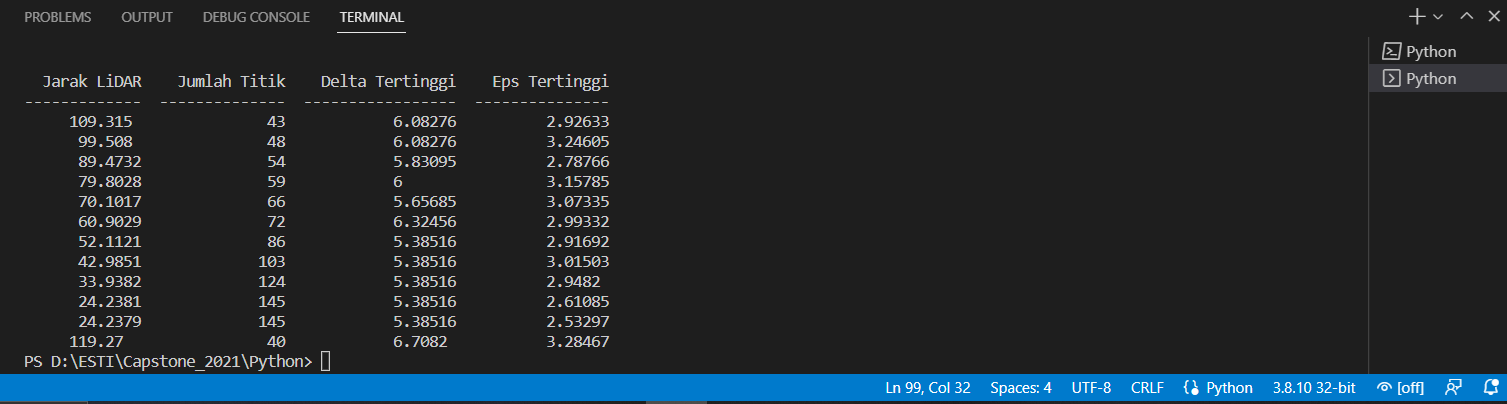
\includegraphics[scale=0.4]{bab5/seed_line_vars.png}
    \caption{Hasil Pengujian \textit{Seed Detection}}
        \label{fig:Ch05_vars_seed}
\end{figure}

Hasil pengujian ditampilkan pada Gambar \ref*{fig:Ch05_vars_seed}. Terlihat bahwa untuk pendeteksian dalam radius 1 m, jumlah titik yang paling sedikit terbaca berjumlah 8 titik untuk segmen lingkaran dan 43 titik untuk segmen garis. Jumlah titik ini dipengaruhi oleh panjang garis, radius lingkaran, dan jarak \lidar. Pembacaan nilai radius lingkaran dalam jarak hingga 1 m memiliki \textit{error} tertinggi pada pembacaan di jarak 90 cm, di bawah jarak tersebut \textit{error} bernilai kurang dari 0,5 cm. Nilai $\delta$ tertinggi yang diperoleh kedua pengujian adalah 7,2111 cm sementara untuk $\epsilon$ adalah 7,62549 cm. Hal ini berarti program yang dibuat dalam sistem deteksi harus memiliki nilai lebih dari nilai variabel yang teruji dengan jumlah titik \textit{seed} tidak lebih dari 8 titik agar sistem dapat mendeteksi segmen garis dan lingkaran. 

\subsection{Skenario Pengujian \textit{Segment Detection} dan Analisis}
\label{subsec:Skenario54}

Pengujian \textit{segment detection} dilakukan dengan menjalankan simulasi robot berjalan dalam ruangan dari ujung kiri menuju ujung kanan. Hasil bacaan robot dikelompokkan menjadi beberapa segmen untuk data yang memenuhi syarat seperti pada Gambar \ref*{fig:Ch05_circ_segment} dengan lingkaran biru besar menunjukkan posisi robot. Robot akan mendeteksi segmen di sekitarnya yang berjarak $\pm$1 m dengan robot. Segmen yang terdeteksi ditampilkan secara \textit{real-time}. 

\begin{figure}[H]
    \centering    
    \begin{subfigure}[b]{.7\linewidth}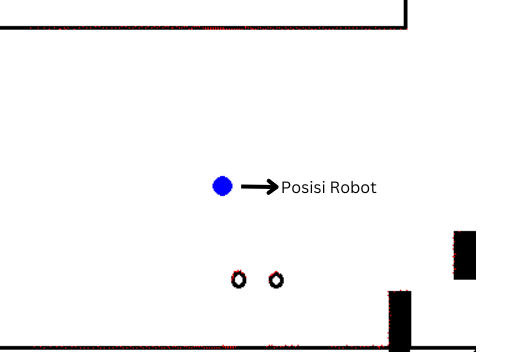
\includegraphics[width=\linewidth]{bab5/position.png}\caption{Posisi Robot di Denah}\label{Fig:Ch05_segmen1}\end{subfigure}
    \hfill
    \vfill
    \begin{subfigure}[b]{.45\linewidth}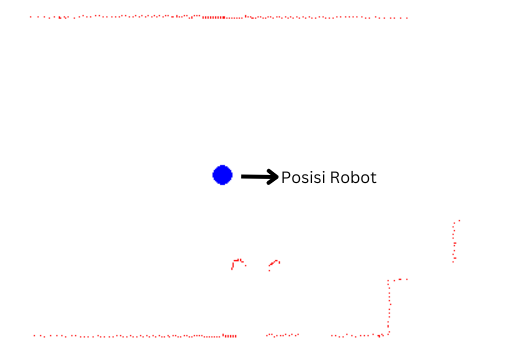
\includegraphics[width=\linewidth]{bab5/point2.png}\caption{Titik Terbaca}\label{Fig:Ch05_segmen2}\end{subfigure}
    \begin{subfigure}[b]{.45\linewidth}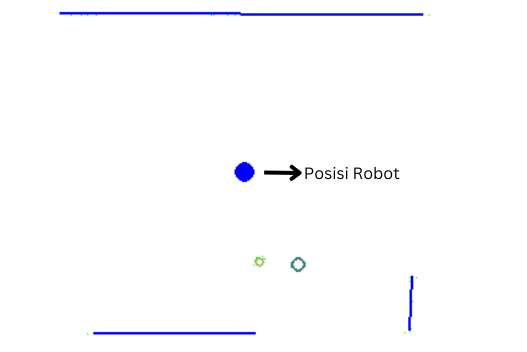
\includegraphics[width=\linewidth]{bab5/garis.png}\caption{Segmen Terbaca}\label{Fig:Ch05_segmen3}\end{subfigure}
    \caption{Pendeteksian \textit{Circle Segment} dan \textit{Line Segment}}
        \label{fig:Ch05_circ_segment}
\end{figure}

Analisis lebih lanjut perlu dilakukan untuk pendeteksian lingkaran karena segmen lingkaran akan digunakan untuk mendeteksi posisi manusia. Beberapa perhitungan digunakan untuk mengetahui kualitas deteksi segmen lingkaran adalah sebagai berikut,
\begin{align}
    \label{eqn:Akurasi}
    &Akurasi\ Pendeteksian = \frac{Jumlah\ Lingkaran\ Terdeteksi\ dengan\ Benar}{Jumlah\ Seluruh\ Lingkaran\ Terdeteksi}\times100\%\\
    &Akurasi\ Posisi =100\%-\frac{Jarak\ Pusat\ Terdeteksi\ dengan\ Pusat\ Asli}{Jarak\ Robot\ dengan\ Pusat\ Asli}\times100\%\\
    &Akurasi\ Radius =100\% - \frac{Jarak\ Radius\ Terdeteksi\ dengan\ Radius\ Asli}{Radius\ Asli}\times100\%.
\end{align}
\begin{figure}[H]
    \centering
    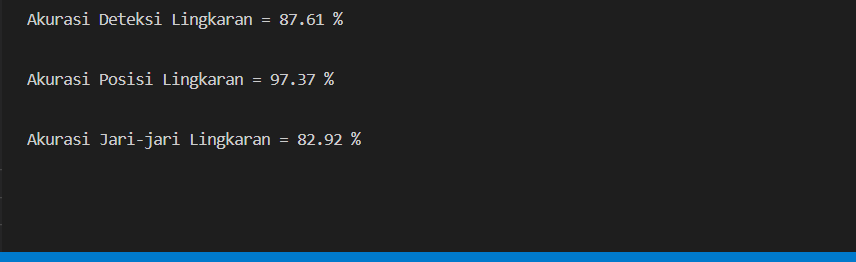
\includegraphics[width=\linewidth]{bab5/hasil.png}
    \caption{Akurasi Pendeteksian Lingkaran}
        \label{fig:Ch05_hasil_akurasi}
\end{figure}
Akurasi yang didapatkan ketika menjalankan simulasi robot bergerak ditunjukkan pada Gambar \ref*{fig:Ch05_hasil_akurasi}. Akurasi berhasil mencapai lebih dari $80\%$ untuk akurasi pendeteksian lingkaran, akurasi posisi, dan akurasi pendeteksian radius lingkaran. Hal ini sudah dapat dianggap mencapai target akurasi yang diinginkan.

\subsection{Skenario Pengujian Klasifikasi dan Simulasi \lidar\ Bergerak dan Analisis}
\label{subsec:Skenario4}
Pengujian terakhir yaitu pengujian simulasi robot berjalan dengan sistem deteksi yang ditambah sistem klasifikasi. Sistem akan mendeteksi garis dan lingkaran kemudian mengelompokkan lingkaran yang memenuhi syarat sebagai kaki manusia. Lingkaran yang terdeteksi sebagai kaki manusia kemudian ditampilkan pada layar dengan bingkai  segi empat berwarna merah sebagai indikator posisi manusia berada pada denah. 
\begin{figure}[H]
    \centering
    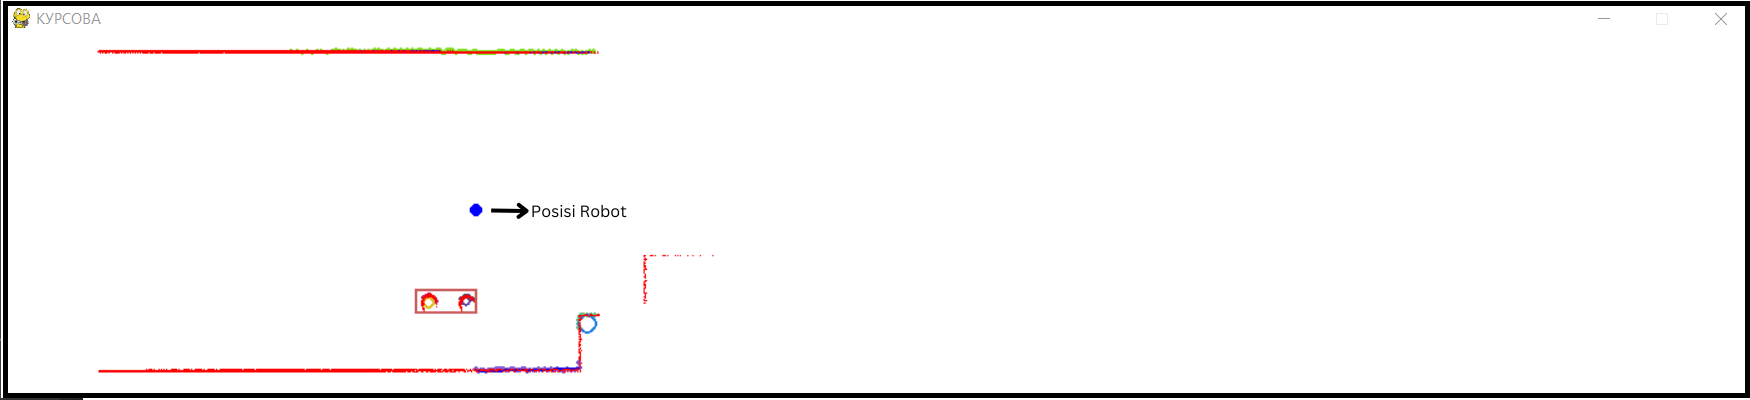
\includegraphics[width=\linewidth]{bab5/simulasi1.png}
    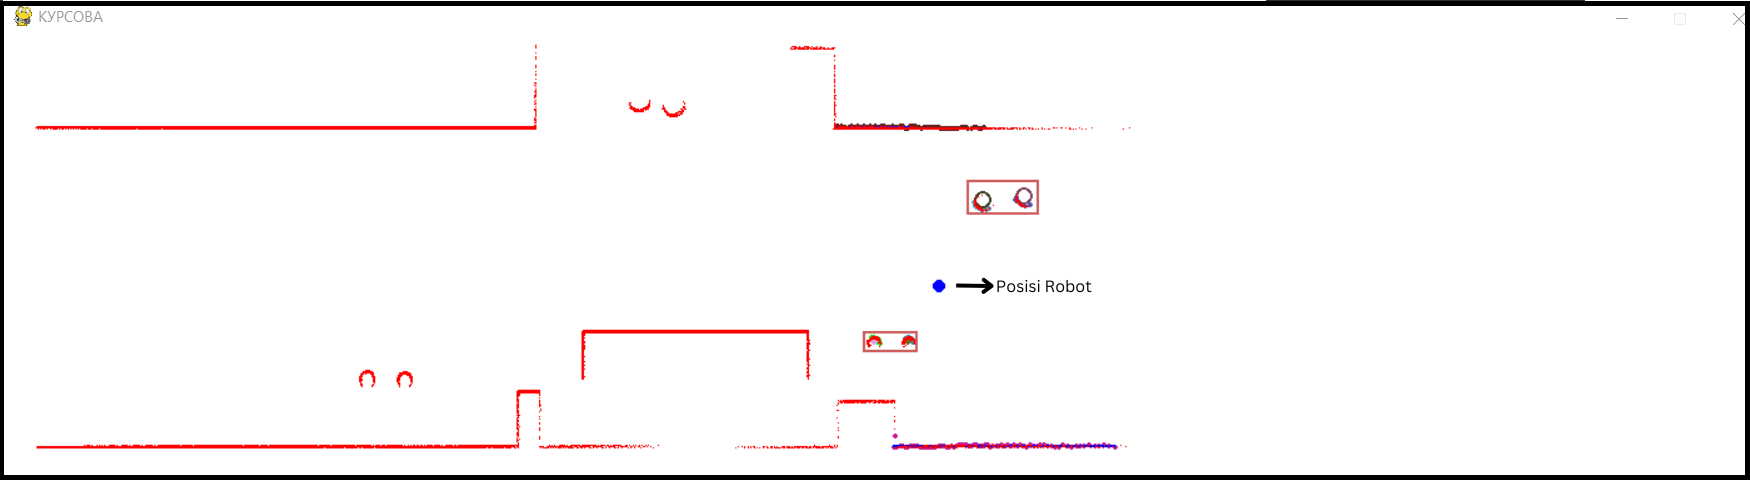
\includegraphics[width=\linewidth]{bab5/simulasi2.png}
    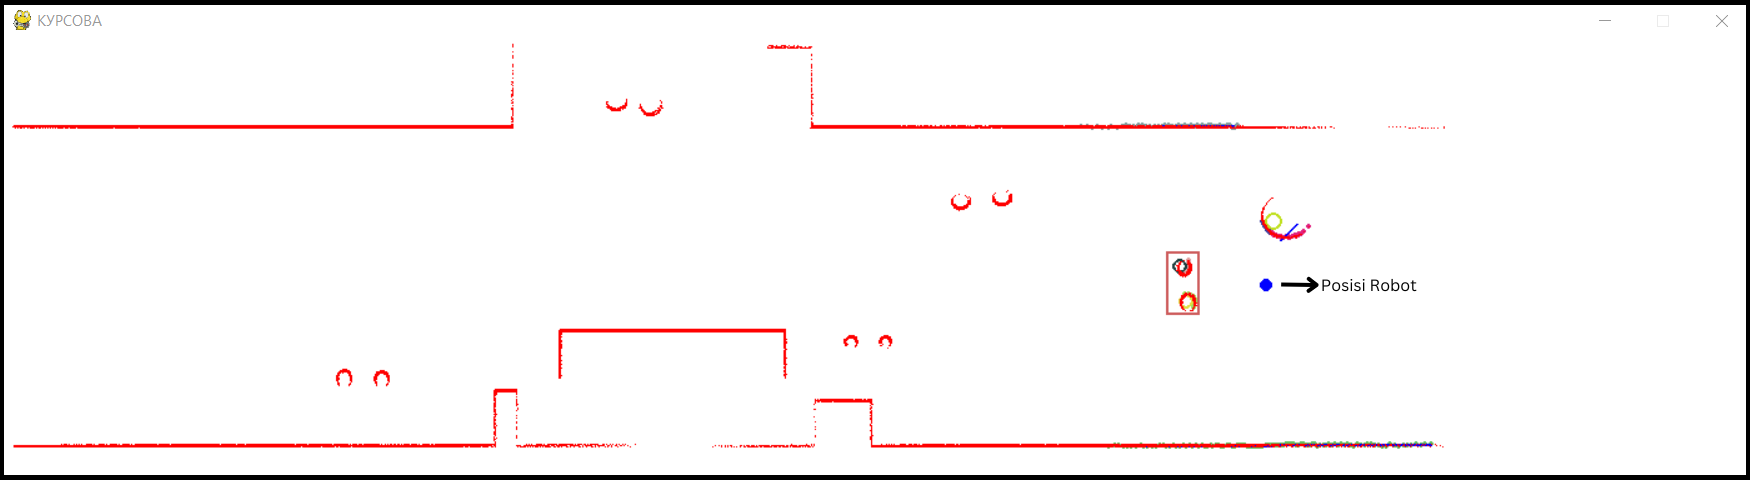
\includegraphics[width=\linewidth]{bab5/simulasi3.png}
    \caption{Simulasi \lidar\ Bergerak dalam Ruangan}
        \label{fig:Ch05_simulasi}
\end{figure}
Uji akurasi juga dilakukan untuk mengetahui keberhasilan klasifikasi manusia pada sistem. Posisi dan ukuran kaki manusia yang sebenarnya digunakan sebagai perbandingan dari posisi yang diketahui sistem. Akurasi pendeteksian manusia dihitung dengan rumus sebagai berikut,
\begin{equation}
    Akurasi=\frac{Jumlah\ Manusia\ Terdeteksi\ Tepat}{Jumlah\ Manusia\ Terdeteksi}.
\end{equation}
\begin{figure}[H]
    \centering
    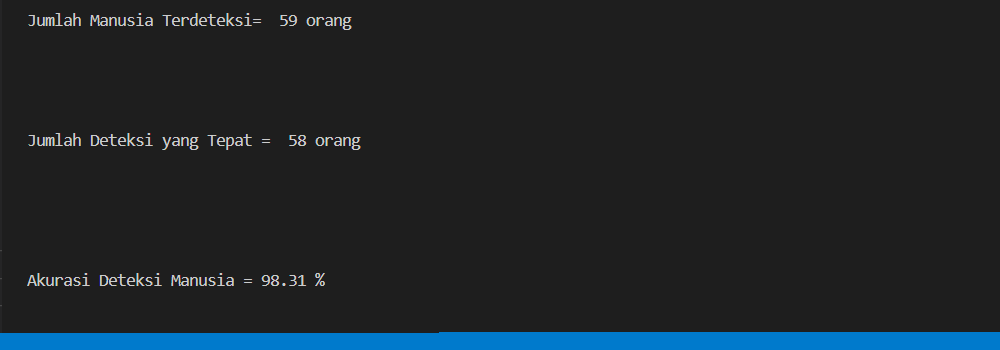
\includegraphics[width=\linewidth]{bab5/akurasi_manusia.png}
    \caption{Uji Akurasi Deteksi Manusia}
        \label{fig:Ch05_akurasi_manusia}
\end{figure}
Hasil pengujian akurasi dapat dilihat pada Gambar \ref*{fig:Ch05_akurasi_manusia}. Satu kali simulasi robot dijalankan dari ujung kiri lorong menuju ujung kanan memperoleh total 59 kali posisi manusia terbaca. Posisi pembacaan yang sesuai dengan denah adalah 58 posisi orang. Terlihat bahwa sistem berhasil mempunyai akurasi diatas $80\%$ yaitu sebesar $98,31\%$, sehingga pendeteksian manusia dapat dianggap memenuhi target yang dirancang.


